\documentclass[twocolumn,apj,numberedappendix,appendixfloats]{openjournal}
% Available options:
% [twocolumn] - two-column mode
% [onecolumn] - (default) main text in one-column mode
% [apj]       - typeset in the style of ApJ.
% [apjl]      - (default) typeset in the style of ApJ Letters 
% [tighten]   - some adjustments to approximate grid typesetting
% [numberedappendix]   - number appendix sections as A, B, etc
% [appendixfloats]  - use separate numbering for floats within appendix
% [twocolappendix]  - make appendix in two-col mode in a two-col paper
%%%%% PACKAGES %%%%%

% Optional useful packages
\usepackage{xcolor}
\usepackage{textgreek}
\usepackage[utf8]{inputenc}
\usepackage[english]{babel}

\usepackage{hyperref}
\hypersetup{
    unicode, 
    colorlinks=true,
    linkcolor=linkcolor,
    citecolor=linkcolor,
    filecolor=linkcolor,
    urlcolor=linkcolor,
}
\usepackage{color,colortbl}
\definecolor{linkcolor}{rgb}{0.0,0.3,0.5}
\usepackage{orcidlink}

% \urlstyle{same}

% Define path to put your plots, figures, etc...
\graphicspath{ {./figures/} }

\begin{document}
\title{Interesting and descriptive title of your research}

\author{\vspace{-1.5cm}YOUR NAME HERE$^{1,*}$}
\author{Sven Buder$^{1,2,*}$\orcidlink{0000-0002-4031-8553}}

% Adding another author would go like:
% \author{FirstName LastName$^{3}$\orcidlink{0000-0000-0000-0000}}

\affiliation{$^{1}$Research School of Astronomy and Astrophysics, Australian National University, Canberra, ACT 2611, Australia}
\affiliation{$^{2}$ARC Centre of Excellence for All Sky Astrophysics in 3 Dimensions (ASTRO 3D), Australia}


\thanks{E-mail: u123456@anu.edu.au}
\thanks{$^*$Australian Research Council DECRA Fellow},

\begin{abstract}
The abstract should include the main content of the paper and make the reader want to actually read the paper. Summarize your work in less than 1920 characters (with spaces) with at least one sentence for each of the following categories:\\
Context (big picture): \\ 
Aims (your hypothesis): \\
Methods: \\
Results: \\
Conclusions (what bigger implications do your findings have):
\end{abstract}

% Write your keywords here
\begin{keywords}
    {Choose up to 6 keywords from \href{https://academic.oup.com/DocumentLibrary/mnras/keywords.pdf}{here} and write them like: keyword1 -- keyword2.}
\end{keywords}

\maketitle


\section{Introduction}
\label{sec:introduction}

The introduction is a condensed version of your literature review. You should start with the bigger picture and tell a story that naturally leads to your hypotheses.

\subsection{Scientific motivation}

You can cite papers in 2 different ways: in-line with parentheses after the authors -- for example for research by \citet{Buder2024} -- or with authors within the parentheses at the end of a statement or paragraph that is backed up by the citation \citep{Buder2024}.

\subsection{Hypotheses}

Here you should clearly point out the hypotheses of your research, that is, the specific questions you want to actually answers. I have found this to be incredibly useful when figuring out how to set up my research and later use these hypotheses as subsection titles for the discussion -- after all: these are the questions that you want to discuss in light of your research. I specifically like to enumerate the hyptotheses (which I phrase as open questions):

\begin{enumerate}
    \item How ...?
    \item How much ...?
    \item When ...?
    \item Which ...?
    \item Where ...?
\end{enumerate}

\subsection{Structure of the paper}

The paper is structured as follows: Section~\ref{sec:data} describes the data of \dots. Section~\ref{sec:analysis} analyses \dots. We discuss our analysis in the context of our hypotheses in Section~\ref{sec:discussion} and bundles our results into an overarching conclusion in Section~\ref{sec:conclusions}.

\clearpage
\section{Data} \label{sec:data}



\clearpage
\section{Analysis} \label{sec:analysis}

Analyses typically include formulae (such as Eq.~\ref{eq:emc2}), tables (such as Tab.~\ref{table:table}), and a lot of nice figures (such as Fig.~\ref{fig:fig}).

\begin{equation}
    E = m c^2 \label{eq:emc2}
\end{equation}

\begin{table}
    \centering
    \caption{Parameters used in your paper.}
    \begin{tabular}{ c c }  
        Parameter & Prior \\
        \hline \hline     
        {\boldmath$\alpha$} & $\left[ 10^{-3}, 10 \right]$ \\
        {\boldmath$\beta$} & $\left[ 0, 1 \right]$ \\   
        \hline \hline  
    \end{tabular}  
    \label{table:table}
\end{table}

\begin{center}
    \begin{figure}[!t]
        \centering
    	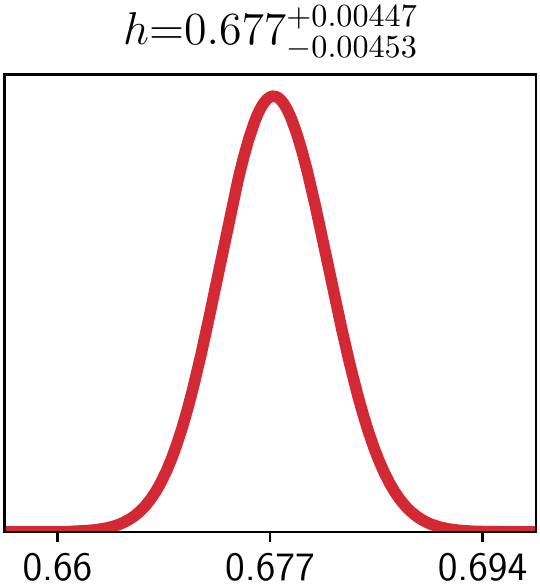
\includegraphics[scale=0.3]{figures/probdist.png}
    	\caption{Nice plot.}
        \label{fig:fig}
    \end{figure}
\end{center}

\clearpage

\section{Discussion} \label{sec:discussion}

\clearpage

\section{Conclusions} \label{sec:conclusions}

\clearpage

\section*{Acknowledgments}

Acknowledge support (or not).

\bibliographystyle{mnras}
\bibliography{bib}

\begin{appendix}

\section{Useful information}



\end{appendix}

\end{document}